
%\begin{figure}[t]
%\centering
%\includegraphics[scale=1,clip]{figure/n2n.eps}\vspace*{-3ex}
% \caption{Merging technique}\vspace*{-3.5ex}
% \label{fig:n2n}
%\end{figure}

\section{Discussion and Future Work}
\label{sec:discuss}

We next discuss issues in our approach and describe how we address
these issues in our future work.

\textbf{Detecting more behavioral difference.} Although our approach detected many behavioral differences, it may fail to reveal all behaviors. To detect more behavioral differences, some directions seem to be promising: (1) we can rely on side effects or  mock objects to test methods without return values; (2) to test API methods that return random values, we can check the distribution of their returned values; (3) other tools such as Cute~\cite{koushik:cute} and JPF~\cite{visser2003mcp} may help generate more test cases to reveal more behaviors. We plan to explore these directions in future work.
%3) to test methods that need to read files, we can generate test cases based on Java Compatibility Kit\footnote{\url{http://jck.dev.java.net}} where standard call sequences and files are prepared;

\textbf{Testing more API elements.} Canfora \emph{et al.}~\cite{CanforaFFT08} propose an approach that can wrap functionalities of legacy system as services. We plan to adapt their wrappers to test mapped API elements across different types of languages in future work. Besides, our approach does not cover some API elements in the same language (\emph{e.g.}, abstract classes and protected elements). To test these elements, we plan to extend our wrappers in future work (\emph{e.g.}, generating a concrete wrapper class for each abstract class).

\textbf{Testing translation of code structures.} As shown in our evaluations, translation tools may fail to translate if code structures are complicated. Daniel \emph{et al.}~\cite{daniel2007automated} propose an approach that tests refactoring engines by comparing their refactored results given the same generated abstract syntax trees. In future work, we plan to adapt their approach to test translation tools by comparing their translation results given the same code structures as inputs.

%\textbf{Testing API mapping of single language.} We find that many existing approaches translate applications within single languages. For example, twinning~\cite{nita2010using} translates applications based on mapping relations of API invocations from different API libraries, and CatchUp!~\cite{henkel2005catchup} translates applications based on mapping relations of API invocations from different versions. In future work, we plan to adapt our approach to test mapping relations of API invocations within single languages. 